\documentclass[a4paper, 12pt]{article}
\usepackage[top=2cm, bottom=2cm, left=2.5cm, right=2.5cm]{geometry}
\usepackage[utf8]{inputenc}
\usepackage[T1]{fontenc}
\usepackage[portuguese]{babel}
\usepackage{indentfirst}
\usepackage{graphicx}
\usepackage{float}
\usepackage{amsmath}

\usepackage{subcaption}
\usepackage{hyperref}


\usepackage[backend=bibtex]{biblatex}
\addbibresource{referencias.bib}

\usepackage{comment}


\title{Modelos matemáticos para identificar o perfil 3d de superfícies digitalizados por meio da visão monocular com projeção de luz estruturada}
\author{Elisângela Ribeiro, Fernando Pujaico Rivera, Bianca Batista Barreto,\\Roberto Alves Braga Junior, Marco Antônio Barbosa 
\\elismar1952@hotmail.com; fernando.pujaico.rivera@gmail.com;
\\biabarreto89@gmail.com; robbraga@gmail.com; marco.fisioedu@ufla.br}


\begin{document}
\maketitle

%%%%%%%%%%%%%%%%%%%%%%%%%%%%%%%%%%%%%%%%%%%%%%%%%%%%%%%%%%%%%%%%%%%%%%%%%%%%%%%%
%%%%%%%%%%%%%%%%%%%%%%%%%%%%%%%%%%%%%%%%%%%%%%%%%%%%%%%%%%%%%%%%%%%%%%%%%%%%%%%%
%%%%%%%%%%%%%%%%%%%%%%%%%%%%%%%%%%%%%%%%%%%%%%%%%%%%%%%%%%%%%%%%%%%%%%%%%%%%%%%%
\section*{Resumo}
Uma imagem é a representação visual de um objeto real em uma superfície sensível gerada a partir de um foco central. 
Esta pode variar de acordo com os dados intrínsecos da câmera e da geometria da cena. 
Sendo a luz estruturada um processo de projetar um padrão conhecido em uma cena, a forma como o padrão se deforma quando atinge a superfície permite que sistemas de visão calculem a profundidade e informações das superfícies dos objetos na cena. 
Partindo desse pressuposto, este trabalho tem o objetivo de identificar o perfil de um objeto em um plano de referência, a partir de dados intrínsecos da câmera, da geometria da cena e da luz estruturada, por meio de visão monocular. 
Para isso foi desenvolvido uma função de correção envolvendo modelos matemáticos para identificar todos os parâmetros que compõem o sistema gerador da imagem. 
Esse sistema é composto pelas variáveis de entrada de acordo com a configuração experimental. 
Os resultados mostraram que foi possível identificar as distorções dos eixos X, Y e Z e traçar o perfil do objeto em análise em três dimensões.


\textbf{Palavra-chave:}  Luz estruturada; perfil; três dimensões.

%%%%%%%%%%%%%%%%%%%%%%%%%%%%%%%%%%%%%%%%%%%%%%%%%%%%%%%%%%%%%%%%%%%%%%%%%%%%%%%%
%%%%%%%%%%%%%%%%%%%%%%%%%%%%%%%%%%%%%%%%%%%%%%%%%%%%%%%%%%%%%%%%%%%%%%%%%%%%%%%%
%%%%%%%%%%%%%%%%%%%%%%%%%%%%%%%%%%%%%%%%%%%%%%%%%%%%%%%%%%%%%%%%%%%%%%%%%%%%%%%%
\section*{Abstract}

An image is the visual representation of a real object on a sensitive surface generated from a central focus. 
This can vary according to the intrinsic data of the camera and scene geometry. 
Being structured light is a process of projecting a known pattern in a scene, the way the pattern deforms when it reaches the surface allows vision systems to calculate the depth and information of the surfaces of objects in the scene. 
Based on this assumption, this work aims to identify the profile of an object in a reference plane, using intrinsic data from the camera, the geometry of the scene and structured light, through monocular vision. 
For this purpose, a correction function was developed involving mathematical models to identify all the parameters that make up the image generating system. 
This system is composed of the input variables according to the experimental configuration. 
The results showed that it was possible to identify the distortions of the X, Y and Z axes and to profile the object under analysis in three dimensions.

\textbf{Keywords:}Structured light; profile; three dimensions. 


%%%%%%%%%%%%%%%%%%%%%%%%%%%%%%%%%%%%%%%%%%%%%%%%%%%%%%%%%%%%%%%%%%%%%%%%%%%%%%%%
%%%%%%%%%%%%%%%%%%%%%%%%%%%%%%%%%%%%%%%%%%%%%%%%%%%%%%%%%%%%%%%%%%%%%%%%%%%%%%%%
%%%%%%%%%%%%%%%%%%%%%%%%%%%%%%%%%%%%%%%%%%%%%%%%%%%%%%%%%%%%%%%%%%%%%%%%%%%%%%%%
\section{Introdução}

Aqui vem o texto


%%%%%%%%%%%%%%%%%%%%%%%%%%%%%%%%%%%%%%%%%%%%%%%%%%%%%%%%%%%%%%%%%%%%%%%%%%%%%%%%
%%%%%%%%%%%%%%%%%%%%%%%%%%%%%%%%%%%%%%%%%%%%%%%%%%%%%%%%%%%%%%%%%%%%%%%%%%%%%%%%
%%%%%%%%%%%%%%%%%%%%%%%%%%%%%%%%%%%%%%%%%%%%%%%%%%%%%%%%%%%%%%%%%%%%%%%%%%%%%%%%
\section{Material e Métodos}

Os procedimentos metodológicos para a execução do projeto seguiram os seguintes passos:

\begin{itemize}
\item Montagem da configuração experimental (ver Seção \ref{subsec:montagem}).
\item Digitalização de uma superfície (ver Seção \ref{subsec:digitaliza}).
\item Binarização de uma imagem em cores (ver Seção \ref{subsec:binariza}).
\item Obtendo uma linha em 3D a partir de imagens em 2D (ver Seção \ref{subsec:obtendolinha}).
\item Otimizando experimentalmente os valores dos parâmetros (ver Seção \ref{subsec:otimizandopar}). 
\end{itemize}

Todos os experimentos foram realizados nas dependências da Universidade Federal de Lavras (UFLA), 
dividido entre os laboratórios nº 2 e 7 do Centro de Desenvolvimento à Instrumentação aplicado à Agropecuária (CEDIA), 
ligado ao Departamento de Automática.

A configuração experimental foi elaborada por meio da visão monocular \cite{RIBEIRO:2014} com projeção de Luz estruturada para a digitalização de várias superfícies.
Nessa configuração, com o auxílio do projetor conectado ao computador, 
projetam-se linhas horizontais sobre o objeto em análise, de forma a identificar o delineamento da superfície.

\begin{figure}[h!]
	\centering
		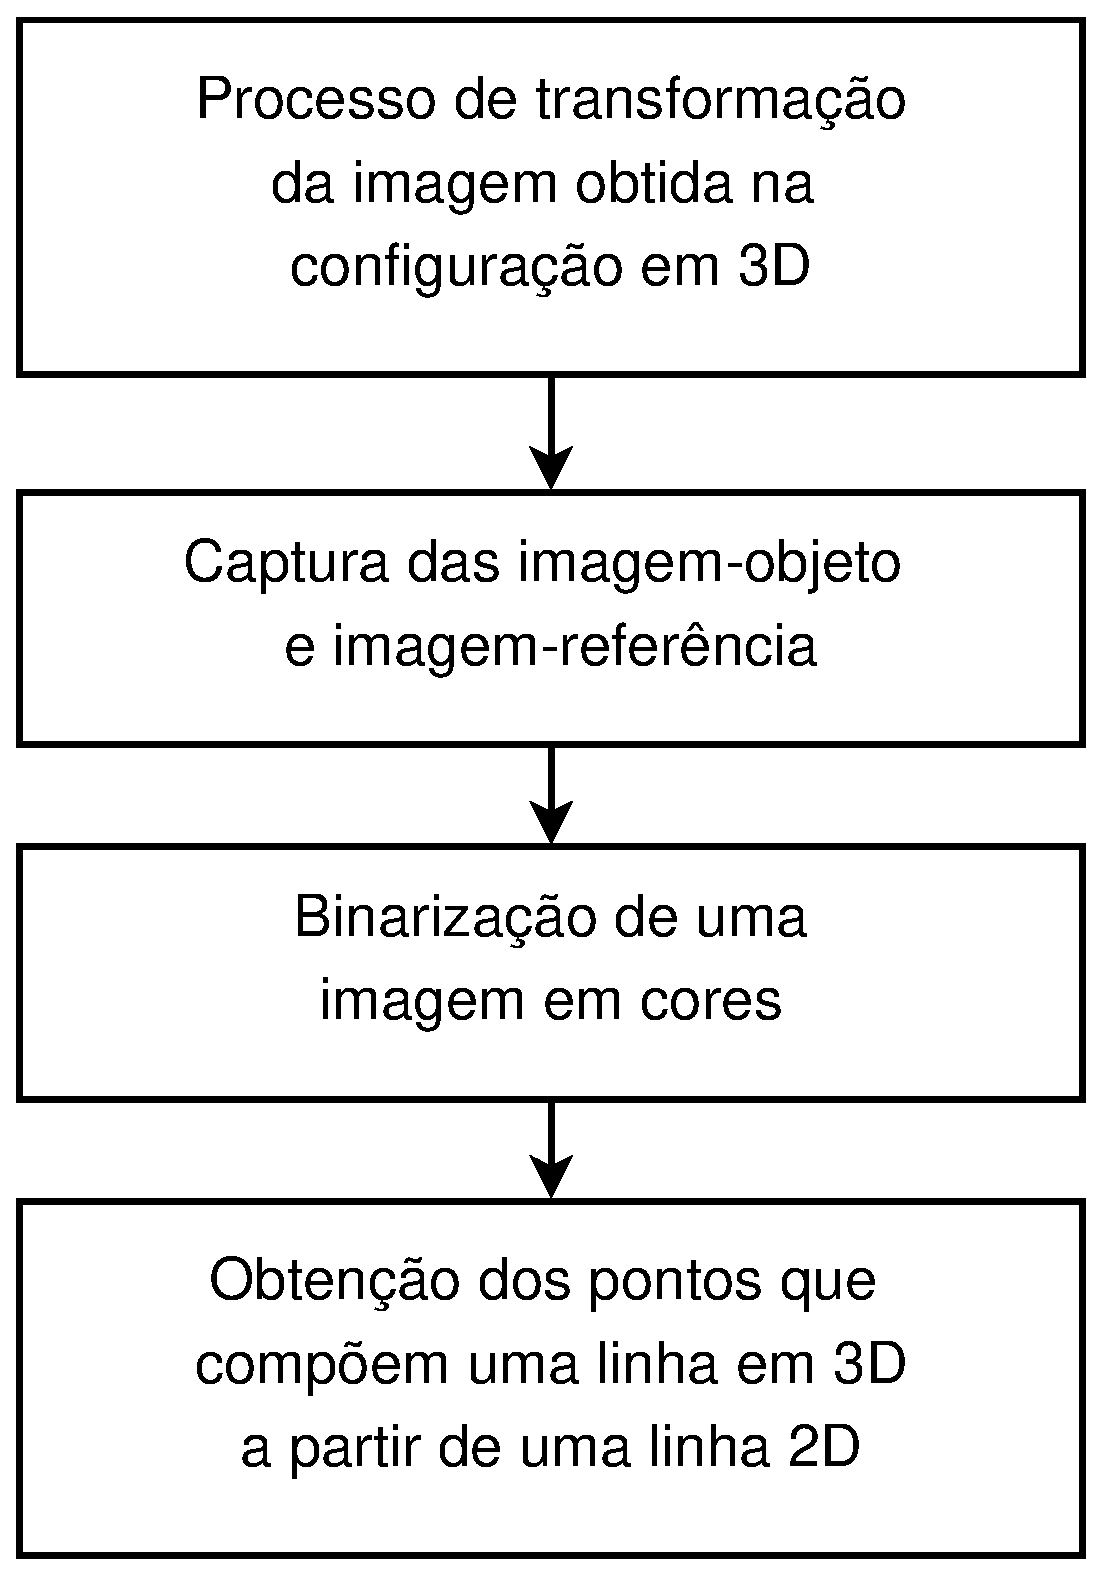
\includegraphics[width=.35\linewidth]{fluxograma_identificar_3D.eps}
	\caption{Fluxograma para identificar o perfil 3D}
	\label{fluxograma_identificar_3D}
\end{figure}


No fluxograma da Figura \ref{fluxograma_identificar_3D}, é responsável pelo procedimento de transformação da imagem obtida na configuração em 3D, o qual primeiramente teve como objetivo apresentar o processo de transformação da imagem digitalizada, na configuração experimental, a uma representação em 3D. Para isso, foi necessário a captura das imagens objeto e referência com a projeção das linhas coloridas sobre as costas humana. Em seguida, foi desenvolvido um algoritmo para a binarização de uma imagem em cores.

%%%%%%%%%%%%%%%%%%%%%%%%%%%%%%%%%%%%%%%%%%%%%%%%%%%%%%%%%%%%%%%%%%%%%%%%%%%%%%%%
\subsection{Montagem da configuração experimental}
\label{subsec:montagem}

Para a configuração do sistema, utilizou-se de uma fonte de luz como o projetor e apenas uma câmera, ambos dispostos em ângulos em relação ao objeto, ilustrado na Figura \ref{arranjo-experimetal}, conhecido também como Luz estruturada (projeção de um padrão conhecido – como linhas horizontais que ao tocar o objeto desenha a sua superfície) por meio da visão monocular (utiliza apenas uma câmera).

\begin{figure}[h!]
\centering
    \begin{subfigure}{.695\textwidth}
      \centering
      % include first image
      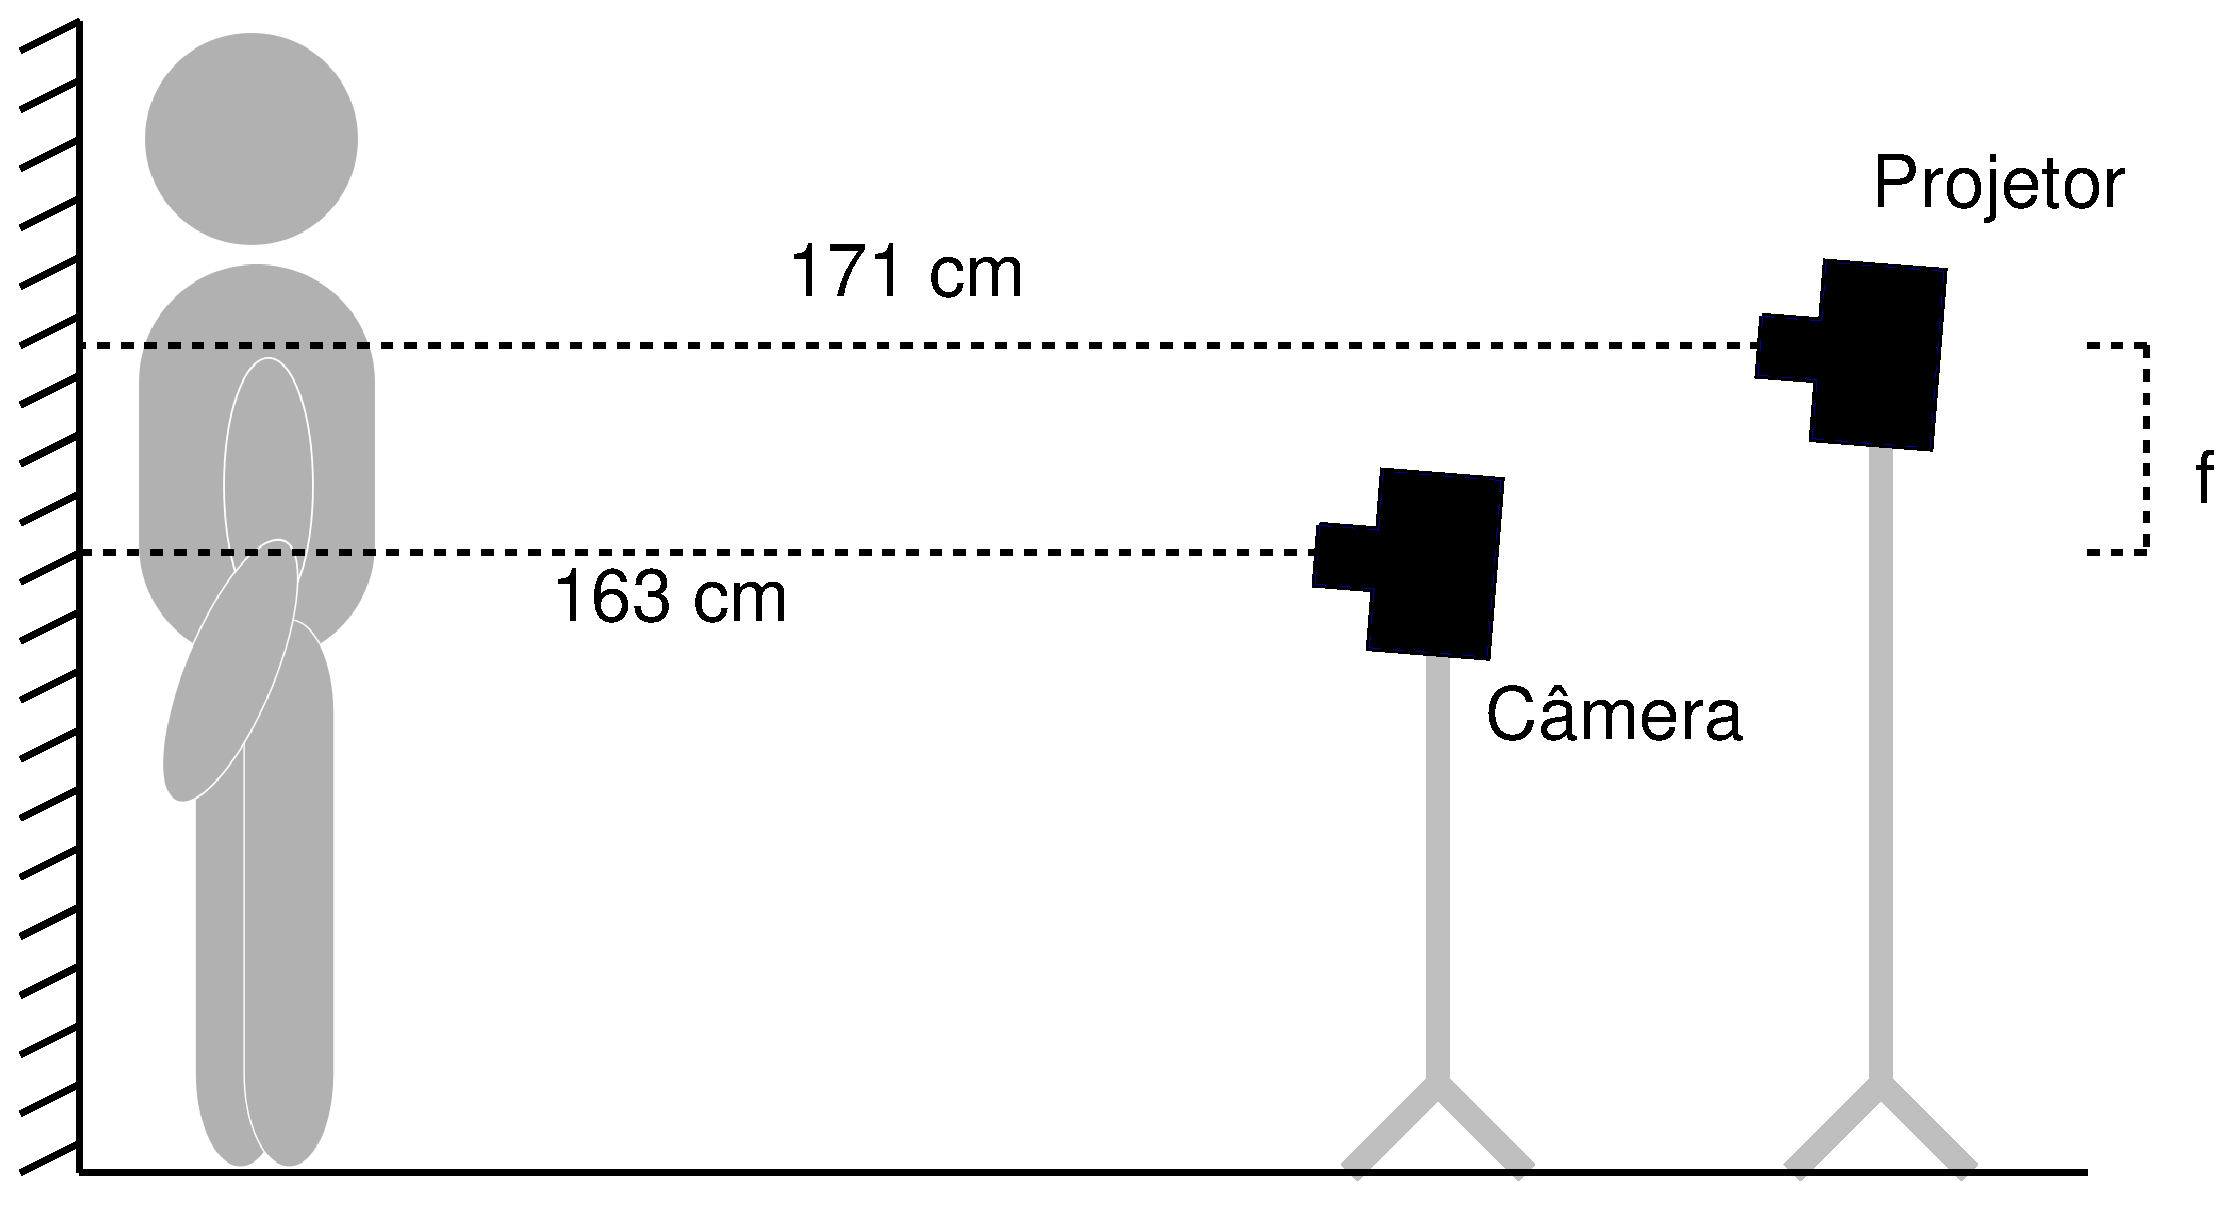
\includegraphics[width=.95\linewidth]{configuracao_sistema_1.eps}  
      \caption{Disposição do arranjo experimental}
      \label{arranjo-experimetal:1}
    \end{subfigure}
    \begin{subfigure}{.295\textwidth}
      \centering
      % include first image
      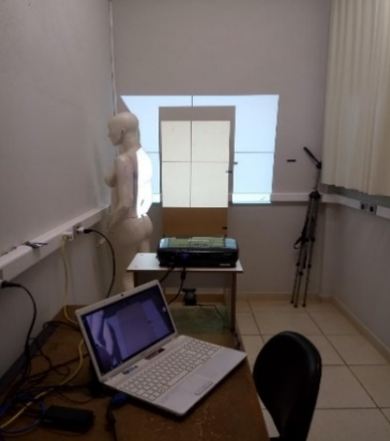
\includegraphics[width=.95\linewidth]{configuracao_sistema_2.png}
      \caption{Fotografia do arranjo experimental}
      \label{arranjo-experimetal:2}
    \end{subfigure}	
\caption{Arranjo experimental utilizando luz estruturada}
\label{arranjo-experimetal}
\end{figure}


Os equipamentos utilizados na configuração experimental foram: uma webcam com as seguintes configurações: Hd, 3.0 Mb, Usb da marca Logitech C270 960-000691, um projetor multimídia Benq com as seguintes descrições: Mx525b 3200 Lumens/Xga/Hdmi/3D Ready/Bndes e um computador portátil Sony Vaio Core i3. 

Na configuração, a fonte de luz ficou fixada a uma distância de 171 cm do objeto. A câmera ficou fixada a uma distância de 136 cm do objeto, conforme ilustra a Figura \ref{arranjo-experimetal}.  Com a utilização de um computador portátil conectado ao projetor, projetaram linhas sobre o objeto.

Ao montar a configuração experimental utilizando visão monocular, foi possível identificar várias variáveis no setup, conforme ilustra a Figura \ref{setup com as variaveis} a seguir.

\begin{figure}[h!]
	\centering
		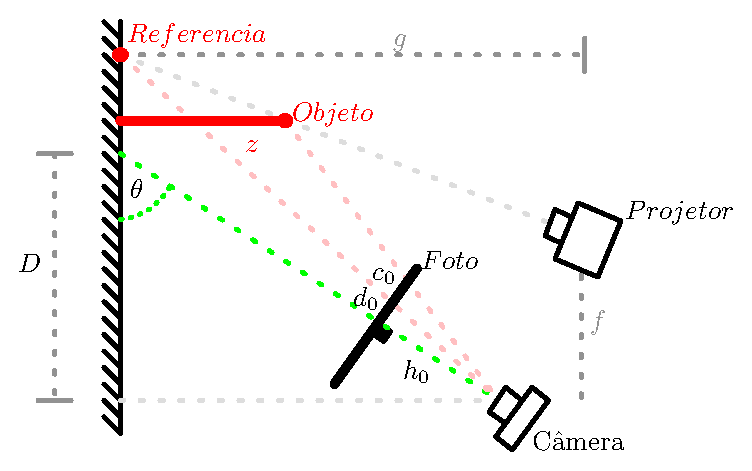
\includegraphics[width=.55\linewidth]{Diagrama1.eps}
	\caption{Variáveis da Configuração Experimental em uma vista sagital}
	\label{setup com as variaveis}
\end{figure}

Sendo:

\begin{itemize}
\item g: Medida em centímetros da altura do projetor em relação ao plano de referência;
\item f:  Distância em centímetros entre o projetor e a câmera;	          
\item $\theta$: Ângulo formado entre a câmera e o plano de referência;
\item $h_0$: Distância focal em pixels da câmera em relação ao objeto;  
\item D:  Distância em centímetros entre sigma e beta;
\item C: Altura real do objeto, também identificado pela variável z;
\item $c_0$: Altura relativa em pixels do objeto na imagem digitalizada;
\item $d_0$: Diferença em pixels entre o ponto central real da imagem até a linha de referência projetada, sendo que esses dados estão em referência na fotografia digitalizada. 
\end{itemize} 
 
Todas essas variáveis foram importantes para o desenvolvimento de modelos matemáticos utilizados nos algoritmos desenvolvidos. 


%%%%%%%%%%%%%%%%%%%%%%%%%%%%%%%%%%%%%%%%%%%%%%%%%%%%%%%%%%%%%%%%%%%%%%%%%%%%%%%%
\subsection{Digitalização de uma superfície}
\label{subsec:digitaliza}

Com a câmera fixada em um tripé, capturou-se uma foto da projeção da linha sobre o objeto, conforme ilustra a Figura \ref{imagem_projecao_colorida:a}. Em seguida, removeu-se o objeto, e o mesmo procedimento foi repetido para a captura da imagem do plano, conhecida como imagem referência ilustrado na Figura \ref{imagem_projecao_colorida:b}. 

\begin{figure}[h!]
	\centering
    \begin{subfigure}{.35\textwidth}
      \centering
      % include first image
      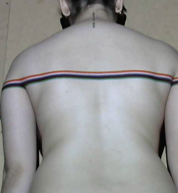
\includegraphics[width=.85\linewidth]{imagem_projecao_colorida_a.png} 
      \caption{Imagem objeto}
      \label{imagem_projecao_colorida:a}
    \end{subfigure}
    \begin{subfigure}{.35\textwidth}
      \centering
      % include first image
      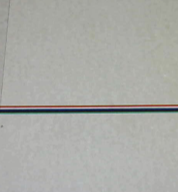
\includegraphics[width=.85\linewidth]{imagem_projecao_colorida_b.png} 
      \caption{Imagem referência}
      \label{imagem_projecao_colorida:b}
    \end{subfigure}
	\caption{Projeção das linhas coloridas}
	\label{imagem_projecao_colorida}
\end{figure}

As linhas projetadas nas costas das pessoas foram coloridas seguindo o padrão RGB \cite{LUKACPLATANIOTIS} associado às cores preta e branca, de forma que uma das cinco cores projetadas fossem visualizadas nas fotos capturadas, pois o conjunto de amostras possuíam uma variedade de tonalidade na cor da pele.

%%%%%%%%%%%%%%%%%%%%%%%%%%%%%%%%%%%%%%%%%%%%%%%%%%%%%%%%%%%%%%%%%%%%%%%%%%%%%%%%
\subsection{Binarização de uma imagem em cores}
\label{subsec:binariza}

Esta Seção foi responsável por transformar as imagens capturadas em apenas linhas (binária), ou seja, deixar em evidência binária somente a linha de melhor delineamento, que no caso das imagens digitalizadas, a cor vermelha foi a que teve o melhor destaque nas costas dos indivíduos.

Para realizar esse processo, um algoritmo baseado em identificação de cores foi desenvolvido. Ele teve como dados de entrada a imagem original digitalizada, na qual o algoritmo percorreu toda ela e identificou a cor desejada e descartou todos as outras, obtendo, assim, como imagem final somente a linha da superfície digitalizada, conforme ilustra a Figura \ref{fig:cordetect}.


\begin{figure}[!h]
     \centering
     \begin{subfigure}[b]{0.35\textwidth}
         \centering
         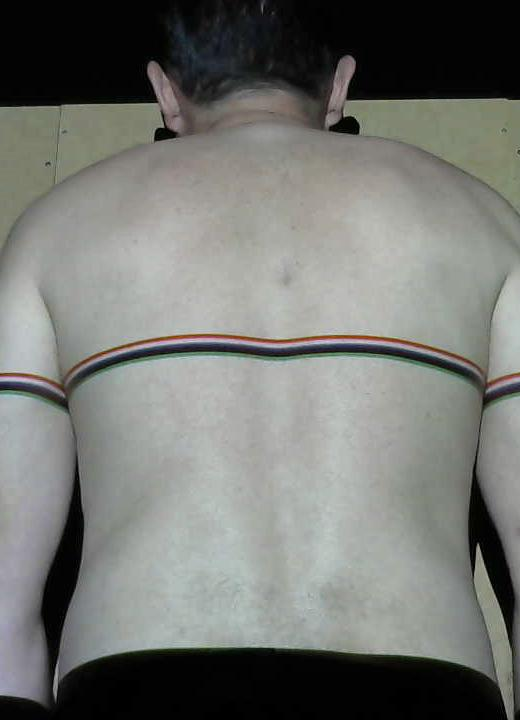
\includegraphics[width=0.85\textwidth]{11_obj_color.jpg}
         \caption{Imagem $\mathbf{A}$ em RGB.}
         \label{fig:cordetect:rgb}
     \end{subfigure}
     \begin{subfigure}[b]{0.35\textwidth}
         \centering
         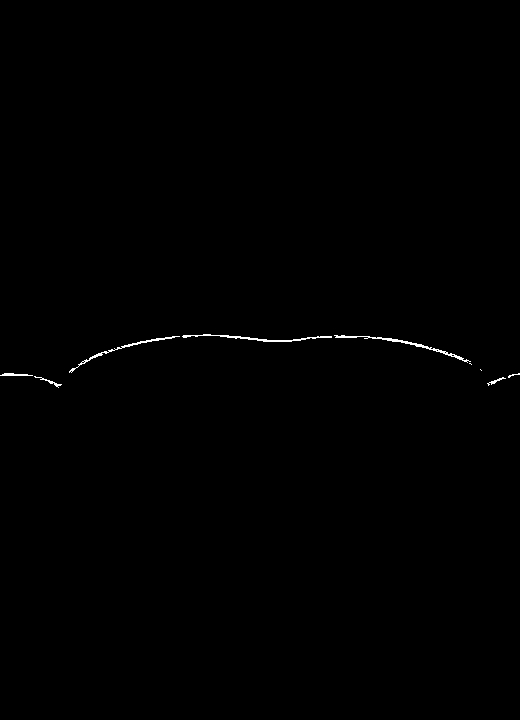
\includegraphics[width=0.85\textwidth]{grayscale.jpg}
         \caption{Imagem $\mathbf{D}$ em BW.}
         \label{fig:cordetect:bw}
     \end{subfigure}
\caption{Processo para identificação da linha na imagem digitalizada}
\label{fig:cordetect}
\end{figure}

\subsubsection{Lógica matemática na identificação de linha}

Conhecida uma imagem $\textbf{A}$ com $L$ pixels codificados 
em RGB (como na Figura \ref{fig:cordetect:rgb}), onde $a_l=(r_l,g_l,b_l)\in \mathbb{R}^3$
representa o pixel $l$, $\forall~1\leq l\leq L$ em $\textbf{A}$, 
de modo que
$r_l$ indica o valor da componente em vermelho do pixel,
$g_l$ indica o valor da componente em verde do pixel e
$b_l$ indica o valor da componente em azul do pixel.
Definimos um detector de cores mediante a função $func\_compare$ descrita na Equação (\ref{eq:funccompare1}),
\begin{equation}\label{eq:funccompare1}
func\_compare(\mathbf{a},\mathbf{c},\epsilon)=
\left\{
\begin{matrix}
1 & if   & \frac{||\mathbf{a}-\mathbf{c}||}{||\mathbf{c}||}<|\epsilon|\\
0 & else & ~
\end{matrix}
\right.,
\end{equation}
que recebe como entrada os vetores $\mathbf{a}$ e $\mathbf{c}$ 
(representando pixeis), e se procura se estes tem uma diferença relativa menor a $|\epsilon|$, 
em caso afirmativo, é dizer se os vetores são semelhantes, se retorna $1$ em caso contrario se retorna $0$.
Na Equação (\ref{eq:funccompare1}) o operador $||\mathbf{c}||$ indica a norma euclidiana de $\mathbf{c}$.


Assim, para obter a linha detetada em branco e preto da Figura \ref{fig:cordetect:bw} 
a partir da linha projetada em cores da Figura \ref{fig:cordetect:rgb}, 
é utilizada a função $func\_compare()$, de modo que primeiro selecionamos um pixel $\mathbf{a}_c$ na imagem $\mathbf{A}$,
representando este pixel a cor a detetar, e logo comparamos
cada pixel $\mathbf{a}_l \in \mathbf{A}$, obtendo como resultado desta comparação $\mathbf{d}_l$, é dizer
\begin{equation}\label{eq:funccompare2}
\mathbf{d}_l\leftarrow func\_compare(\mathbf{a}_l,\mathbf{a}_c,\epsilon),\quad \forall~ 1\leq l\leq L,
\end{equation}
apos estes cálculos os valores $\mathbf{d}_l$ são ordenados para formar a imagem $\mathbf{D}$, 
como exemplifica a Figura \ref{fig:cordetect:bw}, onde a cor branca representa um 
valor $1$ e a cor preta um valor $0$.
No caso da Figura \ref{fig:cordetect} é usado o valor $\epsilon=0.25$.



%%%%%%%%%%%%%%%%%%%%%%%%%%%%%%%%%%%%%%%%%%%%%%%%%%%%%%%%%%%%%%%%%%%%%%%%%%%%%%%%
\subsection{Obtendo uma linha em 3D a partir de imagens em 2D}
\label{subsec:obtendolinha}

Nesta seção é mostrado como a partir de duas imagens binarias, 
uma referente a um objeto iluminado com luz estruturada,
e outra da mesma luz iluminando um plano de referencia;
podemos obter uma curva em 3D que representa a altura de um objeto em estudo em relação
ao plano de referencia.
\begin{figure}[!h]
     \centering
     \begin{subfigure}[b]{0.5\textwidth}
         \centering
         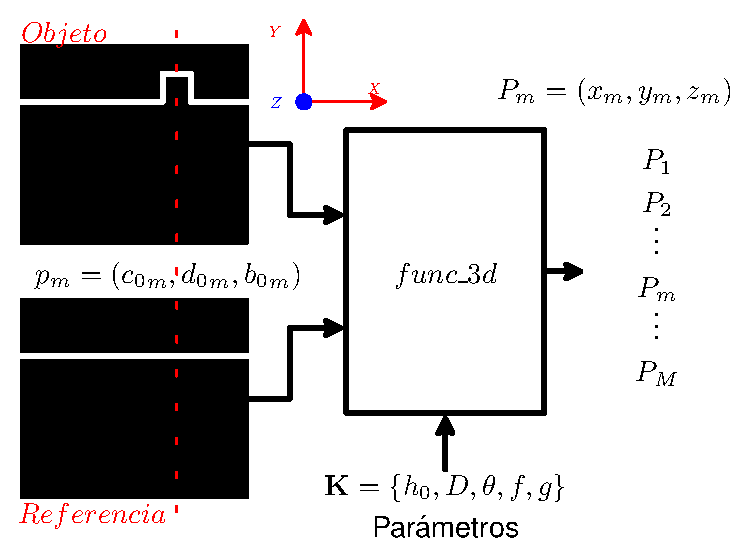
\includegraphics[width=\textwidth]{Diagrama3.eps}
         \caption{Diagrama de blocos.}
         \label{fig:blocos:sys}
     \end{subfigure}
     \hfill
     \begin{subfigure}[b]{0.425\textwidth}
         \centering
         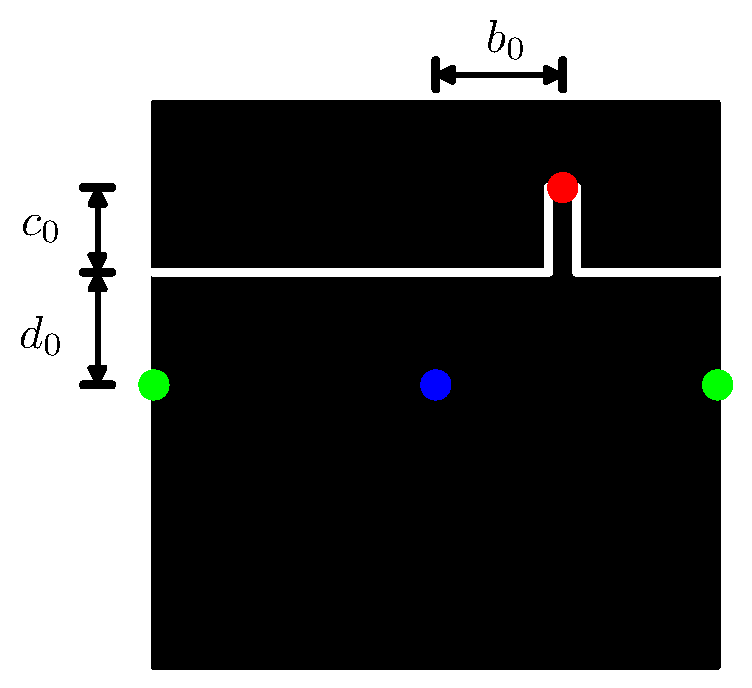
\includegraphics[width=\textwidth]{Diagrama2.eps}
         \caption{Objeto em estudo.}
         \label{fig:blocos:obj}
     \end{subfigure}
\caption{Obtendo uma linha em 3D.}
\label{fig:blocos}
\end{figure}
Podemos ver todo este processo resumido na Figura \ref{fig:blocos:sys},
onde são extraídos $M$ pontos $p_m$ (em 2D) das imagens binarias 
e são convertidos em pontos $P_m$ (em 3D),
mediante a função $func\_3d()$ 
\begin{equation}
P \leftarrow func\_3d(p;\mathbf{K}),
\end{equation}
\begin{equation}
p=(c_0,d_0,b_0)\quad \xrightarrow[\mathbf{K}]{func\_3d} \quad P=(x,y,z),
\end{equation}
\begin{equation}
p_m=({c_0}_m,{d_0}_m,{b_0}_m)\quad \xrightarrow[\mathbf{K}]{func\_3d}\quad P_m=(x_m,y_m,z_m).
\end{equation}

Os pontos $p_m$ são extraídos um por cada coluna das imagens binarias,
e estão referenciados ao centro da imagem, é dizer os valores em $p_m$ podem ser positivos ou negativos.
A Figura \ref{fig:blocos:obj} mostra como são selecionados os valores $(c_0,d_0,b_0)$ para um ponto $p$,
que está ressaltado com um circulo vermelho na imagem. 
O centro da imagem está representado com um circulo azul.
O valor $d_0$ representa a distancia vertical de um ponto da linha de referencia ao centro da imagem,
o valor $c_0$ representa a distancia vertical de um ponto da linha do objeto à linha de referencia, e
o valor $b_0$   representa a distancia horizontal de um ponto da linha do objeto ao centro da imagem.

Os parâmetros do sistema $\mathbf{K}\equiv \{h_0,D,\theta,f,g\}$ são agrupado num vetor $\mathbf{K}$,
e estos valores são extraídos da geometria do sistema; 
por este motivo estes valores não mudam para todos os pontos $p_m$, $\forall~ 1\leq m \leq M$.
A Figura \ref{setup com as variaveis} mostra uma vista sagital da disposição do sistema,
onde as variáveis $h_0$, $D$, $\theta$, $f$ e $g$ são obtidas. 
Dado que a vista é sagital somente são mostradas aqui os valores $y$ e $z$
de um ponto $P=(x,y,z)$;
onde $z$ representa  altura do objeto e 
$y$ a distancia vertical da base do objeto em estudo ao ponto no plano de referencia a onde aponta a câmera;
este ponto é considerada a posição $(0,0,0)$ em 3D.


A função $func\_3d()$ calcula a altura $z$ de um ponto mediante as
Equações (\ref{eq:setup1}) e (\ref{eq:setup2}),
\begin{equation}\label{eq:setup1}
z=\frac{
D~tg(\theta)
\left[
1+ ctg\left(\theta+atg\left(\frac{h_0}{d_0+c_0}\right)\right) ctg\left(\theta-atg\left(\frac{d_0}{h_0}\right)\right) 
\right]
}{
\left[1+ctg\left(\theta+atg\left(\frac{h_0}{d_0+c_0}\right)\right) ctg(\alpha)\right]
},
\end{equation}
\begin{equation}\label{eq:setup2}
ctg(\alpha)=\frac{D~tg(\theta)ctg\left(\theta-atg\left(\frac{d_0}{h_0}\right)\right)- f}{g}.
\end{equation}

O valor $y$ de um ponto analisado pode ser calculado mediante as
Equações (\ref{eq:setup3}) e (\ref{eq:setup2}),
\begin{equation}\label{eq:setup3}
y=D~tg(\theta)ctg\left(\theta-atg\left(\frac{d_0}{h_0}\right)\right)-D-z~ctg(\alpha).
\end{equation}

Para obter o valor $x$ são criadas as variáveis temporais $\gamma$ e $\beta$, como mostra 
a Figura \ref{fig:blocos2:sagital}.
Se geramos um plano com um angulo $\gamma$
obtemos uma vista onde a variável $x$ está evidente, como mostra a Figura \ref{fig:blocos2:plano}.
\begin{figure}[!h]
     \centering
     \begin{subfigure}[b]{0.475\textwidth}
         \centering
         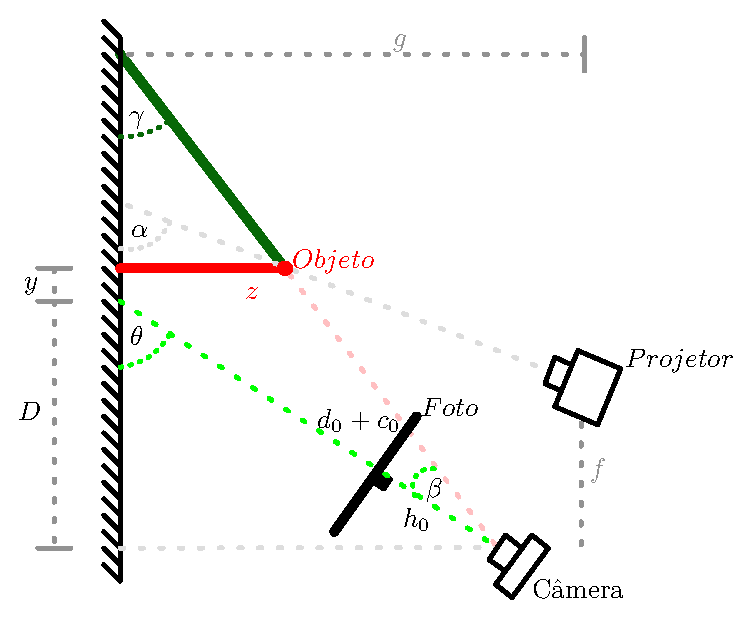
\includegraphics[width=\textwidth]{Diagrama5.eps}
         \caption{Vista sagital do sistema.}
         \label{fig:blocos2:sagital}
     \end{subfigure}
     \hfill
     \begin{subfigure}[b]{0.475\textwidth}
         \centering
         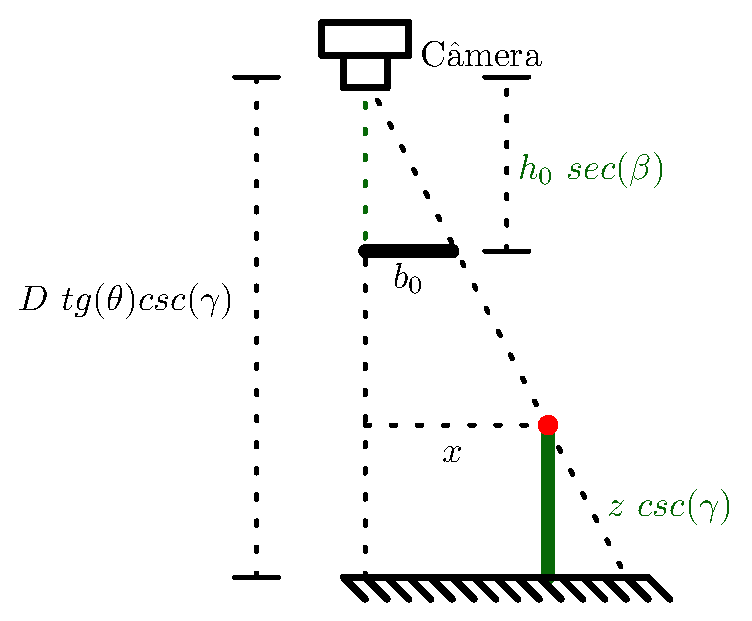
\includegraphics[width=\textwidth]{Diagrama4.eps}
         \caption{Vista do plano com angulo $\gamma$.}
         \label{fig:blocos2:plano}
     \end{subfigure}
\caption{Detecção de cores.}
\label{fig:blocos2}
\end{figure}
Destas figuras concluímos que a variável $x$ pode ser obtida das Equações (\ref{eq:setup2:x}), 
 (\ref{eq:setup2:gamma}) e (\ref{eq:setup2:beta})
\begin{equation}\label{eq:setup2:x}
x=b_0\left(\frac{D~tg(\theta)-z}{h_0}\right)\left(\frac{csc\left({\gamma}\right) }{\sec\left(\beta\right)}\right),
\end{equation}
\begin{equation}\label{eq:setup2:gamma}
\gamma=\theta-\beta,
\end{equation}
\begin{equation}\label{eq:setup2:beta}
\beta=atg\left(\frac{c_0+d_0}{h_0}\right).
\end{equation}

\subsubsection{Calculando a altura $z$}
Para obter a altura $z$ de um objeto a partir de um valor $c_0$ 
extraído de uma imagem em 2D, é usada a função
$func\_z(c_0;\mathbf{K})$, 
\begin{equation}
z = func\_z(c_0;\mathbf{K}),
\end{equation}
\begin{equation}\label{eq:setupz1}
func\_z(c_0;\mathbf{K})\equiv\frac{
D~tg(\theta)
\left[
1+ ctg\left(\theta+atg\left(\frac{h_0}{d_0+c_0}\right)\right) ctg\left(\theta-atg\left(\frac{d_0}{h_0}\right)\right) 
\right]
}{
\left[1+ctg\left(\theta+atg\left(\frac{h_0}{d_0+c_0}\right)\right) \left(\frac{D~tg(\theta)ctg\left(\theta-atg\left(\frac{d_0}{h_0}\right)\right)- f}{g}\right)\right]
},
\end{equation}
sendo $\mathbf{K}=[d_0,h_0,D,\theta,f,g]^T$
um vetor que contem os parâmetros que não modificam seu valor em todos os analises,
pois pertencem à geometria do sistema implementado (setup).
Assim, se conhecemos o vetor $\mathbf{K}$, o cálculo da altura $z$, mediante a função $func\_z()$,
depende unicamente da variável $c_0$.
Porém o cálculo dos parâmetros em $\mathbf{K}$ mediante medições de alturas e ângulos
é um trabalho laborioso que traz muitos erros de medida.
Pelo que em vez de tentar obter ou medir os parâmetros em $\mathbf{K}$,
aqui se optou por realizar a seguinte aproximação da função $func\_z()$, 
mediante a função $f_{\mathbf{P}}()$, 
\begin{equation}
func\_z(c_0;\mathbf{K})\equiv f_{\mathbf{P}}(c_0),
\end{equation}
que representa una serie de Taylor,
\begin{equation}
\begin{align*}
f_{\mathbf{P}}(c_0)  &\equiv p_0+p_1~c_0+p_2~c_0^2+p_3~c_0^3+...\\ 
 &\equiv \sum_{i=0}^{\infty}p_i~c_0^i
\end{align*}
\end{equation}
na qual, o vetor $\mathbf{P}=[p_0,~p_1,~p_2,~...]$ tem infinitos elementos. 
O parâmetro $p_0$ é fácil de aproximar pois se assume que $f_{\mathbf{P}}(0)\approx 0$,
de modo que $p_0\approx 0$ e 
\begin{equation}
f_{\mathbf{P}}(x)  \equiv p_1~x+p_2~x^2+p_3~x^3+...
\end{equation}
a partir de aqui realizamos uma aproximação considerando a geometria do sistema
e testes para identificar o erro desta aproximação. Finalmente foi observado
que um polinômio de primeiro ordem (quer dizer $p_i=0|\forall i\geq 2$) 
já produzia uma aproximação adequada à altura real dos objetos,
pelo que agora  
\begin{equation}
func\_z(c_0;\mathbf{K})\equiv f_{\mathbf{P}}(c_0)\approx p_1 c_0;
\end{equation}
assim, o único parâmetro desconhecido é $p_1$.
\begin{remark}
É importante ressaltar que esta é uma aproximação,
pelo que se houvéssemos escolhido
$func\_z(c_0;\mathbf{K}) \approx p_0 + p_1 c_0+p_2 c_0^2$,
poderíamos ter atingido reconstruções mais apuradas,
porém a aproximação de primeiro ordem já cumpre com o objetivo.
\end{remark}

Assim, usando a função $f_{\mathbf{P}}(c_0)$ podemos achar a altura $z$
a partir do valor $c_0$ numa fotografia, como mostra a Figura \ref{fig:blocos:obj}.
Lembrando que $c_0$ é a medida de diferencia da altura entre de um objeto na fotografia
e a linha de referencia numa posição $d_0$.


Por outro lado, para obter o valor $p_1$ é usado um objeto de tamanho $z$ conhecido,
ao qual se lhe toma uma fotografia e se obtém o valor $c_0$;
assim, para obter o valor $p_1$ usamos,
\begin{equation}
p_1=\frac{z}{c_0}.
\end{equation}
\begin{remark}
Para aprimorar mais o cálculo de $p_1$ também poderiam ser tomadas varias amostras
$d_n=\{z^{(n)},c_0^{(n)}\}$, para todo inteiro $n$ que cumpra $1\leq n \leq N$.
De modo que $p_1=E\left[\frac{z^{(n)}}{c_0^{(n)}}\right]$, 
sendo que $E[.]$ representa ao operador esperança.
\end{remark}


%%%%%%%%%%%%%%%%%%%%%%%%%%%%%%%%%%%%%%%%%%%%%%%%%%%%%%%%%%%%%%%%%%%%%%%%%%%%%%%%
\subsection{Otimizando experimentalmente os valores dos parâmetros}
\label{subsec:otimizandopar}
Nesta Seção, foi desenvolvido o sistema representado na Figura \ref{sitema_otimizacao}, o qual foi composto por cinco variáveis ($h_0$, D, $\theta$, f e g), e seus parâmetros foram possíveis de serem identificados de forma manual que, eventualmente, possui erro devido à imprecisão de medição humana. Porém, é necessário que esses parâmetros sejam o mais real possível, sendo necessário realizar uma aproximação desses dados.

\begin{figure}[h!]
	\centering
		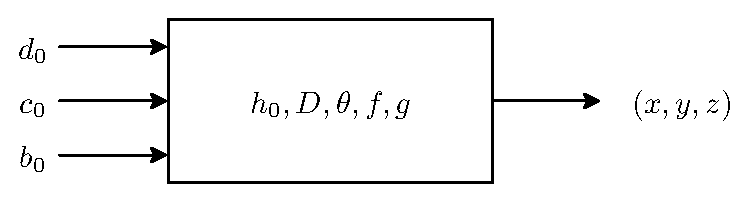
\includegraphics[width=.55\linewidth]{sitema_otimizacao.eps}
	\caption{Sitema para otimizar parâmetros}
	\label{sitema_otimizacao}
\end{figure}

Utilizando o software Octave, foi possível desenvolver um algoritmo que fosse capaz de otimizar os dados inseridos manualmente e retornar o melhor valor da medição com o menor erro possível. Baseado nos passos descritos no fluxograma da Figura \ref{identificar parametros}, foi possível realizar essa aproximação dos dados.


\begin{figure}[h!]
	\centering
		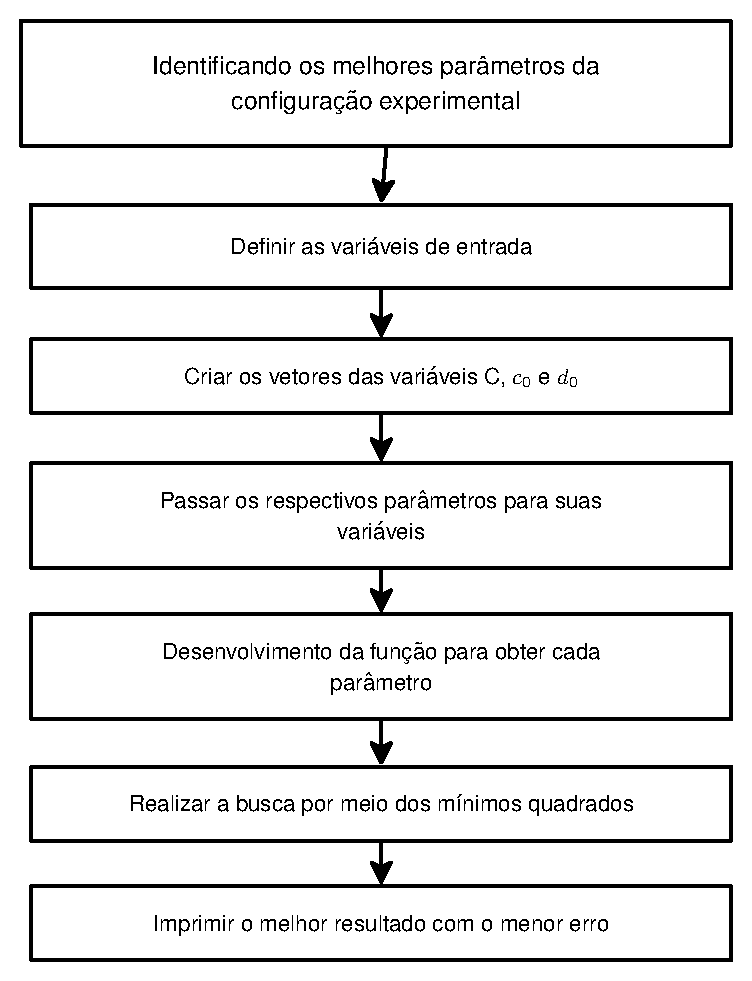
\includegraphics[width=.55\linewidth]{fluxograma_identificar_parametros.eps}
	\caption{Fluxograma para identificar parâmetros}
	\label{identificar parametros}
\end{figure}

Para desenvolver o algoritmo de otimização dos parâmetros, primeiro definiram-se os parâmetros do sistema como sendo $h_0$, D, $\theta$, f e g, para receber os dados calculados manualmente. Logo, foi criado um vetor com o propósito de receber os parâmetros de $c_0$ e $d_0$ que foram calculados do primeiro objeto digitalizado, com o objetivo de otimizar e identificar os melhores parâmetros para z.

Uma função para receber todos os dados da geometria foi desenvolvida. Utilizou-se de cálculos matemáticos baseados no método dos mínimos quadrados, pelo qual se procurou encontrar o melhor ajuste para o conjunto de dados medidos manualmente, tentando minimizar a soma dos quadrados das diferenças entre os valores estimados e os dados medidos manualmente; porém, utilizar parâmetros calculados medidos manualmente apresentou respostas com erros.

Para melhorar os parâmetros medidos manualmente, foi necessário oferecer mais parâmetros de entrada ao sistema da Figura \ref{sitema_otimizacao}; porém, desta vez, recebendo como parâmetros de entrada $c_0$, correspondente às linhas projetadas no plano em relação às mesmas linhas em cima do objeto, $d_0$ correspondente à diferença entre o meio da imagem e à linha de referência no plano e à variável z, como a altura real do objeto.

Com o conjunto de parâmetros f, g, $h_0$, $c_0$, $d_0$ calculados manualmente, realizaram-se as interações com base nos três parâmetros de entrada que retornaram ao melhor valor dos parâmetros do sistema, ou seja, oferecendo os parâmetros certos citados acima, o sistema funcionou perfeitamente, Figura \ref{sitema_otimizacao}. Uma variável E foi inserida ao algoritmo para representar o valor do erro estimado entre as interações feitas nos parâmetros no algoritmo. Essa variável representou que quanto menor o erro, melhor a interação realizada.

Para que a otimização desses parâmetros alcançasse seus melhores resultados, foram utilizados no mínimo 5 grupos de $c_0$, $d_0$ e z, que foram oferecidos em blocos/vetor, pois quanto mais amostras de entrada para z, $c_0$ e $d_0$, melhor os ajustes dos parâmetros e com retorno de valores mais favoráveis para $h_0$, D, $\theta$, f e g. 

\subsubsection{Lógica matemática para otimização dos parâmetros do sistema}

Como já foi visto em seções anteriores, para obter um ponto $P=(x,y,z)$ em 3D a partir de um ponto 
$p=(c_0,d_0,b_0)$ extraído a partir de imagens em 2D, é usada a função
$P \leftarrow func\_3d(p;\mathbf{K})$, sendo $\mathbf{K}=[h_0,D,\theta,f,g]^T$
um vetor que contem os parâmetros da geometria do sistema.
Porem, os valores em $\mathbf{K}\in \mathbb{R}^4$ inicialmente são medidos manualmente,
e precisam ser ajustados a sus valores reais, ou o mais próximos a estos que seja possível;
para cumprir este proposito podemos usar a função $func\_z()$ que é
uma simplificação da função $func\_3d()$ onde 
\begin{equation}
z \leftarrow func\_z(\{c_0,d_0\};\mathbf{K}),
\end{equation}
\begin{equation}
\hat{p}=\{c_0,d_0\}\quad \xrightarrow[\mathbf{K}]{func\_z} \quad z;
\end{equation}
de modo que o cálculo da altura $z$, mediante a função $func\_z()$,
só depende dos valores $\hat{p}=\{c_0,d_0\}$ e $\mathbf{K}$.
\begin{equation}\label{eq:setupz1}
func\_z(\hat{p};\mathbf{K})=\frac{
D~tg(\theta)
\left[
1+ ctg\left(\theta+atg\left(\frac{h_0}{d_0+c_0}\right)\right) ctg\left(\theta-atg\left(\frac{d_0}{h_0}\right)\right) 
\right]
}{
\left[1+ctg\left(\theta+atg\left(\frac{h_0}{d_0+c_0}\right)\right) ctg(\alpha)\right]
},
\end{equation}
\begin{equation}\label{eq:setupz2}
ctg(\alpha)=\frac{D~tg(\theta)ctg\left(\theta-atg\left(\frac{d_0}{h_0}\right)\right)- f}{g}.
\end{equation}
Usando todos estes antecedentes, nosso interesse é encontrar $\mathbf{K}$
com o valor mais ajustado a realidade; é dizer com valores optimizados,
com este fim são processados, e convertidas a imagens binarias, 
um conjunto de objetos de tamanho conhecido,
obtendo $L$ dados $\hat{p}_l$ e $z_l$, $\forall~1\leq l \leq L$.
Onde $z_l$ são as alturas dos objetos e $\hat{p}_l$ 
são os dados extraídos do objeto nas imagens binarias;
com a informação destes dois âmbitos (3D e 2D respetivamente)
definimos a função de custo $e\left(\mathbf{K}\right)$,
\begin{equation}\label{eq:setupz3}
e\left(\mathbf{K}\right)=\sum_{l=1}^{L} \left(z_l-func\_z(\hat{p}_l;\mathbf{K})\right)^2.
\end{equation}
Assim, se os valores $\mathbf{K}$, $\hat{p}_l$ e $z_l$, são medidos ou obtidos de forma exata,
$e\left(\mathbf{K}\right)$ deveria ser igual a zero, devido a que $z_l\approx func\_z(\hat{p}_l;\mathbf{K})$;
porem, como na prática usamos medidas e cálculos aproximados,
nosso objetivo mais eficiente é achar o vetor 
$\mathbf{K}=\mathbf{\bar{K}}$  que minimiza $e\left(\mathbf{K}\right)$.

Para facilitar o cálculo deste mínimo é conveniente expressar a Equação (\ref{eq:setupz3})
na forma matricial como na Equação (\ref{eq:setupz4})
\begin{equation}\label{eq:setupz4}
e\left(\mathbf{K}\right)=|| \mathbf{Z}-\mathbf{F}(\mathbf{K}) ||^2,
\end{equation}
onde $\mathbf{Z}\in \mathbb{R}^L$ é um vetor coluna, 
$\mathbf{F}(\mathbf{K}):\mathbb{R}^4 \rightarrow \mathbb{R}^L$ é uma 
função vetorial de variável vetorial $\mathbf{K}$, e o operador $||.||^2$ indica a norma ao quadrado do vetor,
\begin{equation}
\mathbf{Z}=
\begin{bmatrix}
z_1\\
z_2\\
\vdots\\
z_l\\
\vdots\\
z_L\\
\end{bmatrix},
\qquad
\mathbf{F}(\mathbf{K})=
\begin{bmatrix}
func\_z(\hat{p}_1;\mathbf{K})\\
func\_z(\hat{p}_2;\mathbf{K})\\
\vdots\\
func\_z(\hat{p}_l;\mathbf{K})\\
\vdots\\
func\_z(\hat{p}_L;\mathbf{K})\\
\end{bmatrix}.
\end{equation}
Assim, para minimizar a Equação (\ref{eq:setupz4}) podemos aplicar o
``algoritmo de Levenberg-Marquardt'' (LMA o simplesmente LM), 
tambem conhecido como o ``método de mínimos quadrados amortiguados'' (DLS)
\cite[pp. 232-234]{doicu2010numerical} \cite[pp. 82]{pujaicoriverafernando2020}.
De modo que o vetor $\mathbf{\bar{K}}$ que minimiza a  Equação (\ref{eq:setupz4})
é calculado iterativamente usando a  Equação (\ref{eq:setupz6}) 
\begin{equation}\label{eq:setupz6}
\mathbf{K}_{i+1}\leftarrow\mathbf{K}_{i}+ 
\left[\mathbf{J}(\mathbf{K}_i)^{T}\mathbf{J}(\mathbf{K}_i)+\alpha\mathbf{I}\right]^{-1}
\mathbf{J}(\mathbf{K}_i)^{T}\left[\mathbf{Z}-\mathbf{F}(\mathbf{K}_i)\right],
\end{equation}
onde $\mathbf{I}$ é uma matriz identidade de $4\times 4$, 
a variável $\alpha\geq 0$ é um fator de regularização escolhido por nos,
cujo propósito é conseguir que a matriz 
$\left[\mathbf{J}(\mathbf{K}_i)^{T}\mathbf{J}(\mathbf{K}_i)+\alpha\mathbf{I}\right]$
sempre tenha inversa, e 
 $\mathbf{J}(\mathbf{K})\in \mathbb{R}^{L\times 4}$ é a matriz jacobiana 
\cite[pp. 130]{zhang2017matrix} de $\mathbf{F}(\mathbf{K})$; é dizer
\begin{equation}
\mathbf{J}(\mathbf{K})=\frac{\partial \mathbf{F}(\mathbf{K})}{\partial \mathbf{K}^T}=
\begin{bmatrix}
\frac{\partial func\_z(\hat{p}_1;\mathbf{K})}{\partial \mathbf{K}^T}\\
\frac{\partial func\_z(\hat{p}_2;\mathbf{K})}{\partial \mathbf{K}^T}\\
\vdots\\
\frac{\partial func\_z(\hat{p}_L;\mathbf{K})}{\partial \mathbf{K}^T}\\
\end{bmatrix},
\end{equation}
\begin{equation}\label{eq:setupz9}
\frac{\partial func\_z(\hat{p};\mathbf{K})}{\partial \mathbf{K}^T}\equiv 
\begin{bmatrix}
\frac{\partial func\_z(\hat{p};\mathbf{K})}{\partial h_0} &
\frac{\partial func\_z(\hat{p};\mathbf{K})}{\partial D} &
\frac{\partial func\_z(\hat{p};\mathbf{K})}{\partial \theta} &
\frac{\partial func\_z(\hat{p};\mathbf{K})}{\partial f} &
\frac{\partial func\_z(\hat{p};\mathbf{K})}{\partial g}
\end{bmatrix}.
\end{equation}
Finalmente a Equação (\ref{eq:setupz6}) converge a um vetor $\mathbf{K}_{i+1}$ que é um mínimo global 
de $e\left(\mathbf{K}\right)$, se inciamos o cálculo iterativo desde 
um valor $\mathbf{K}_0$ próximo à solução, neste caso são usados os valores
$\{h_0,D,\theta,f,g\}$ medidos o calculados manualmente. 
As iterações finalizam quando $\mathbf{K}_{i+1}\approx \mathbf{K}_{i}$
onde se declara que o valor ótimo $\mathbf{\bar{K}}\equiv \mathbf{K}_{i+1}$.

Sobre o cálculo das derivadas parciais da função
$func\_z(\hat{p};\mathbf{K})$ em relação a $\mathbf{K}$, como
descrito na Equação (\ref{eq:setupz9}), é fácil observar que estes cálculos
são possíveis porem extremadamente laboriosos;
por este motivo foi usado o motor de cálculo simbólico  
e  sistema de álgebra computacional: Maxima \cite{santos2009introduccao}.
Assim, com a ajuda desse software é calculado de forma simbólica
as derivadas parciais da função $func\_z(\hat{p};\mathbf{K})$ em relação a $\mathbf{K}$.

Todo o processo de optimização antes descrito pode ser sistematizado mediante o diagrama de blocos 
da Figura \ref{fig:Diagrama6}, onde podemos ver 3 entradas de dados e uma saída,
que neste caso é o valor de $\mathbf{K}=\mathbf{\bar{K}}$ que minimiza $e\left(\mathbf{K}\right)$.
\begin{figure}[!h]
     \centering
         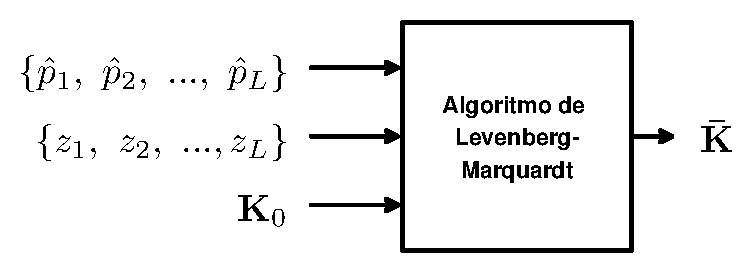
\includegraphics[width=0.5\textwidth]{Diagrama6.eps}
\caption{Algoritmo de Levenberg-Marquardt.}
\label{fig:Diagrama6}
\end{figure}

%%%%%%%%%%%%%%%%%%%%%%%%%%%%%%%%%%%%%%%%%%%%%%%%%%%%%%%%%%%%%%%%%%%%%%%%%%%%%%%%
%%%%%%%%%%%%%%%%%%%%%%%%%%%%%%%%%%%%%%%%%%%%%%%%%%%%%%%%%%%%%%%%%%%%%%%%%%%%%%%%
%%%%%%%%%%%%%%%%%%%%%%%%%%%%%%%%%%%%%%%%%%%%%%%%%%%%%%%%%%%%%%%%%%%%%%%%%%%%%%%%
\section{Resultados e Discussões}

Utilizando apenas uma câmera fixada a uma distância de 136 centímetros em relação ao objeto e a uma altura de 75 centímetros da superfície; um projetor multimídia fixado a uma distância de 171 centímetros do objeto a ser analisado e a uma altura de 112 centímetros da superfície; em seguida, foi possível projetar linhas sobre o objeto de estudo e resultar em seu perfil após o processamento das imagens. A Figura \ref{arranjo-experimetal} ilustra a disposição dos equipamentos, bem como suas respectivas medidas.

%%%%%%%%%%%%%%%%%%%%%%%%%%%%%%%%%%%%%%%%%%%%%%%%%%%%%%%%%%%%%%%%%%%%%%%%%%%%%%%%
%%%%%%%%%%%%%%%%%%%%%%%%%%%%%%%%%%%%%%%%%%%%%%%%%%%%%%%%%%%%%%%%%%%%%%%%%%%%%%%%
%%%%%%%%%%%%%%%%%%%%%%%%%%%%%%%%%%%%%%%%%%%%%%%%%%%%%%%%%%%%%%%%%%%%%%%%%%%%%%%%
\section{Conclusões}


Foi possível desenvolver uma configuração experimental baseada no método interferométrico a partir de apenas uma webcam e um projetor multimídia. 


\printbibliography


\end{document}
